\documentclass{article}


% if you need to pass options to natbib, use, e.g.:
%     \PassOptionsToPackage{numbers, compress}{natbib}
% before loading neurips_2025

\PassOptionsToPackage{numbers, sort, compress}{natbib}

% ready for submission
\usepackage{neurips_2025}


%\bibliographystyle{abbrvnat}
\bibliographystyle{unsrtnat}


\usepackage[pdftex]{graphicx}
\usepackage{amsmath}
% to compile a preprint version, e.g., for submission to arXiv, add add the
% [preprint] option:
%\usepackage[preprint]{neurips_2025}


% to compile a camera-ready version, add the [final] option, e.g.:
%     \usepackage[final]{neurips_2025}


% to avoid loading the natbib package, add option nonatbib:
%    \usepackage[nonatbib]{neurips_2025}


\usepackage[utf8]{inputenc} % allow utf-8 input
\usepackage[T1]{fontenc}    % use 8-bit T1 fonts
\usepackage{hyperref}       % hyperlinks
\usepackage{url}            % simple URL typesetting
\usepackage{booktabs}       % professional-quality tables
\usepackage{amsfonts}       % blackboard math symbols
\usepackage{nicefrac}       % compact symbols for 1/2, etc.
\usepackage{microtype}      % microtypography
\usepackage{xcolor}         % colors

\newcommand\reynotes[1]{\textcolor{purple}{#1}}

%\title{SmokeViz: Using Pseudo-Labels to Develop a Human-Labeled Deep Learning Dataset of Wildfire Smoke Plumes in Satellite Imagery}
\title{SmokeViz: A Large-Scale Satellite Dataset for Wildfire Smoke Detection and Segmentation}


% The \author macro works with any number of authors. There are two commands
% used to separate the names and addresses of multiple authors: \And and \AND.
%
% Using \And between authors leaves it to LaTeX to determine where to break the
% lines. Using \AND forces a line break at that point. So, if LaTeX puts 3 of 4
% authors names on the first line, and the last on the second line, try using
% \AND instead of \And before the third author name.


\author{%
  Rey Koki\\%\thanks{rey.koki@colorado.edu} \\
  Department of Computer Science\\
  University of Colorado Boulder\\
  Boulder, Colorado 80303\\
  \texttt{rey.koki@colorado.edu} \\
  % examples of more authors
  % \And
  % Coauthor \\
  % Affiliation \\
  % Address \\
  % \texttt{email} \\
  % \AND
  % Coauthor \\
  % Affiliation \\
  % Address \\
  % \texttt{email} \\
  % \And
  % Coauthor \\
  % Affiliation \\
  % Address \\
  % \texttt{email} \\
  % \And
  % Coauthor \\
  % Affiliation \\
  % Address \\
  % \texttt{email} \\
}


\begin{document}






\appendix

\section{Supplementary Material}

\section{A. Original Data and Software Licenses}

The HMS smoke product does not have a license attached to it. For GOES imagery, NOAA states: \emph{"There are no restrictions on the use of this data"}. PyTroll is distributed under the GNU General Public License v3.0, and Segmentation Models PyTorch is distributed under the MIT License.

\section{B. Satellite and Band Selection}


As described in the main paper, Advanced Baseline Imager (ABI) bands 1-3 were selected for their high signal-to-noise ratio (SNR) and relevance to visible smoke. Figure \ref{G16_vs_G17} shows an example of GOES-West provides higher visibility of a smoke plume than GOES-East near sunrise. This effect is consistent with Mie scattering physics, where forward-scattered light enhances contrast for aerosols like smoke under favorable solar geometry.

\setcounter{figure}{9}

\begin{figure}[!htb]
    \centering
    \includegraphics[width=\linewidth]{figures/G17_s20221371250321_35.61_-105.01_36.png}
    \caption{(a) True color GOES-EAST (top) and GOES-WEST (bottom) imagery from May \(18^{th}\), 2022 centered at (\(35.6^{\circ}\), \(-105.0^{\circ}\)) in New Mexico, USA taken at 12:50 UTC. The GOES-East and West raw band imagery for (c) blue, (d) red and (e) veggie bands show variations in the SNR for smoke detection in relation to the \(\lambda\) of light being measured.}\label{G16_vs_G17}
\end{figure}

Figure \ref{all_bands} presents a smoke plume in a cloudy scene across all 16 ABI bands described in Table \ref{band_table}. The smoke signal is prominent in Bands 1–3 but diminishes in subsequent NIR channels. Band C07 (3.9 \(\mu\)m), which is sensitive to thermal anomalies, shows a strong fire signal at the source of the plume. While useful for active fire detection, including C07 for smoke segmentation may bias models toward learning fire-smoke co-location, reducing generalization to detached or low opacity smoke plumes, especially those classified as light density that have traveled far from the source. This concern supports the decision to limit input channels in SmokeViz to those that reflect the analyst operational view while minimizing potential modeling shortcuts and dataset size. The SmokeViz dataset development code is designed to be easily adapted to incorporate any desired spectral bands and/or composites.


\begin{figure}[!htb]
    \centering
    \includegraphics[width=\linewidth]{figures/G16_s20221550056176_33_-106_all_band.png}
    \caption{GOES-EAST imagery for all 16 bands from June \(5^{th}\), 2022 centered at (\(33.0^{\circ}\), \(-106.0^{\circ}\)) in New Mexico, USA taken at 00:56 UTC.}\label{all_bands}
\end{figure}

\begin{table}[!htb]
\centering
\caption{The GOES-Series Advanced Baseline Imager (ABI) provides data at 16 channels that cover visible (C01-C02), near-IR (C03-C06) and IR (C07-C16) bands.}
\begin{tabular}{llcc}
\toprule
\textbf{Band} & \textbf{Description} & \textbf{Center Wavelength (\(\mu\)m)} & \textbf{Spatial Resolution (km)} \\
\midrule
C01  & Blue visible                & 0.47     & 1   \\
C02  & Red visible                 & 0.64     & 0.5 \\
C03  & Veggie near IR             & 0.865    & 1   \\
C04  & Cirrus                     & 1.378    & 2   \\
C05  & Snow/Ice                   & 1.61     & 1   \\
C06  & Cloud particle             & 2.24     & 2   \\
C07  & Shortwave IR               & 3.9      & 2   \\
C08  & Upper-level water vapor    & 6.2      & 2   \\
C09  & Mid-level water vapor      & 6.9      & 2   \\
C10  & Lower-level water vapor    & 7.3      & 2   \\
C11  & IR cloud phase             & 8.5      & 2   \\
C12  & Ozone                      & 9.6      & 2   \\
C13  & Clean longwave IR          & 10.35    & 2   \\
C14  & Longwave IR                & 11.2     & 2   \\
C15  & Dirty longwave IR          & 12.3     & 2   \\
C16  & CO\(_2\)                         & 13.3     & 2   \\
\bottomrule
\end{tabular}
\label{band_table}
\end{table}

\subsection{Statistical Dataset Visualizations}

Figures \ref{num_frames}-\ref{count_per_country} summarize key statistical characteristics of the SmokeViz dataset.

Figure \ref{num_frames} presents a histogram of the number of GOES satellite frames associated with each HMS annotation. Since frames are available every 10 minutes, this visualization reflects the variability in annotation time window duration. Most annotations span between 5 and 50 frames, corresponding to 50 minutes to just over 8 hours, underscoring the need for resolving temporal ambiguity during dataset refinement.

Figure \ref{count_per_yr} shows the number of SmokeViz samples per year, stratified by smoke density. The year 2020 exhibits the highest sample count, aligning with an exceptionally active wildfire season across North America \cite{fires2020}. The density distribution across years also varies, with some years showing a higher relative proportion of light or medium smoke annotations.

Lastly, SmokeViz includes annotations across North America, Figure \ref{count_per_country} summarizes the dataset's geographic coverage by country, including the United States, Canada, and Mexico.



\begin{figure}[!htb]
    \centering
        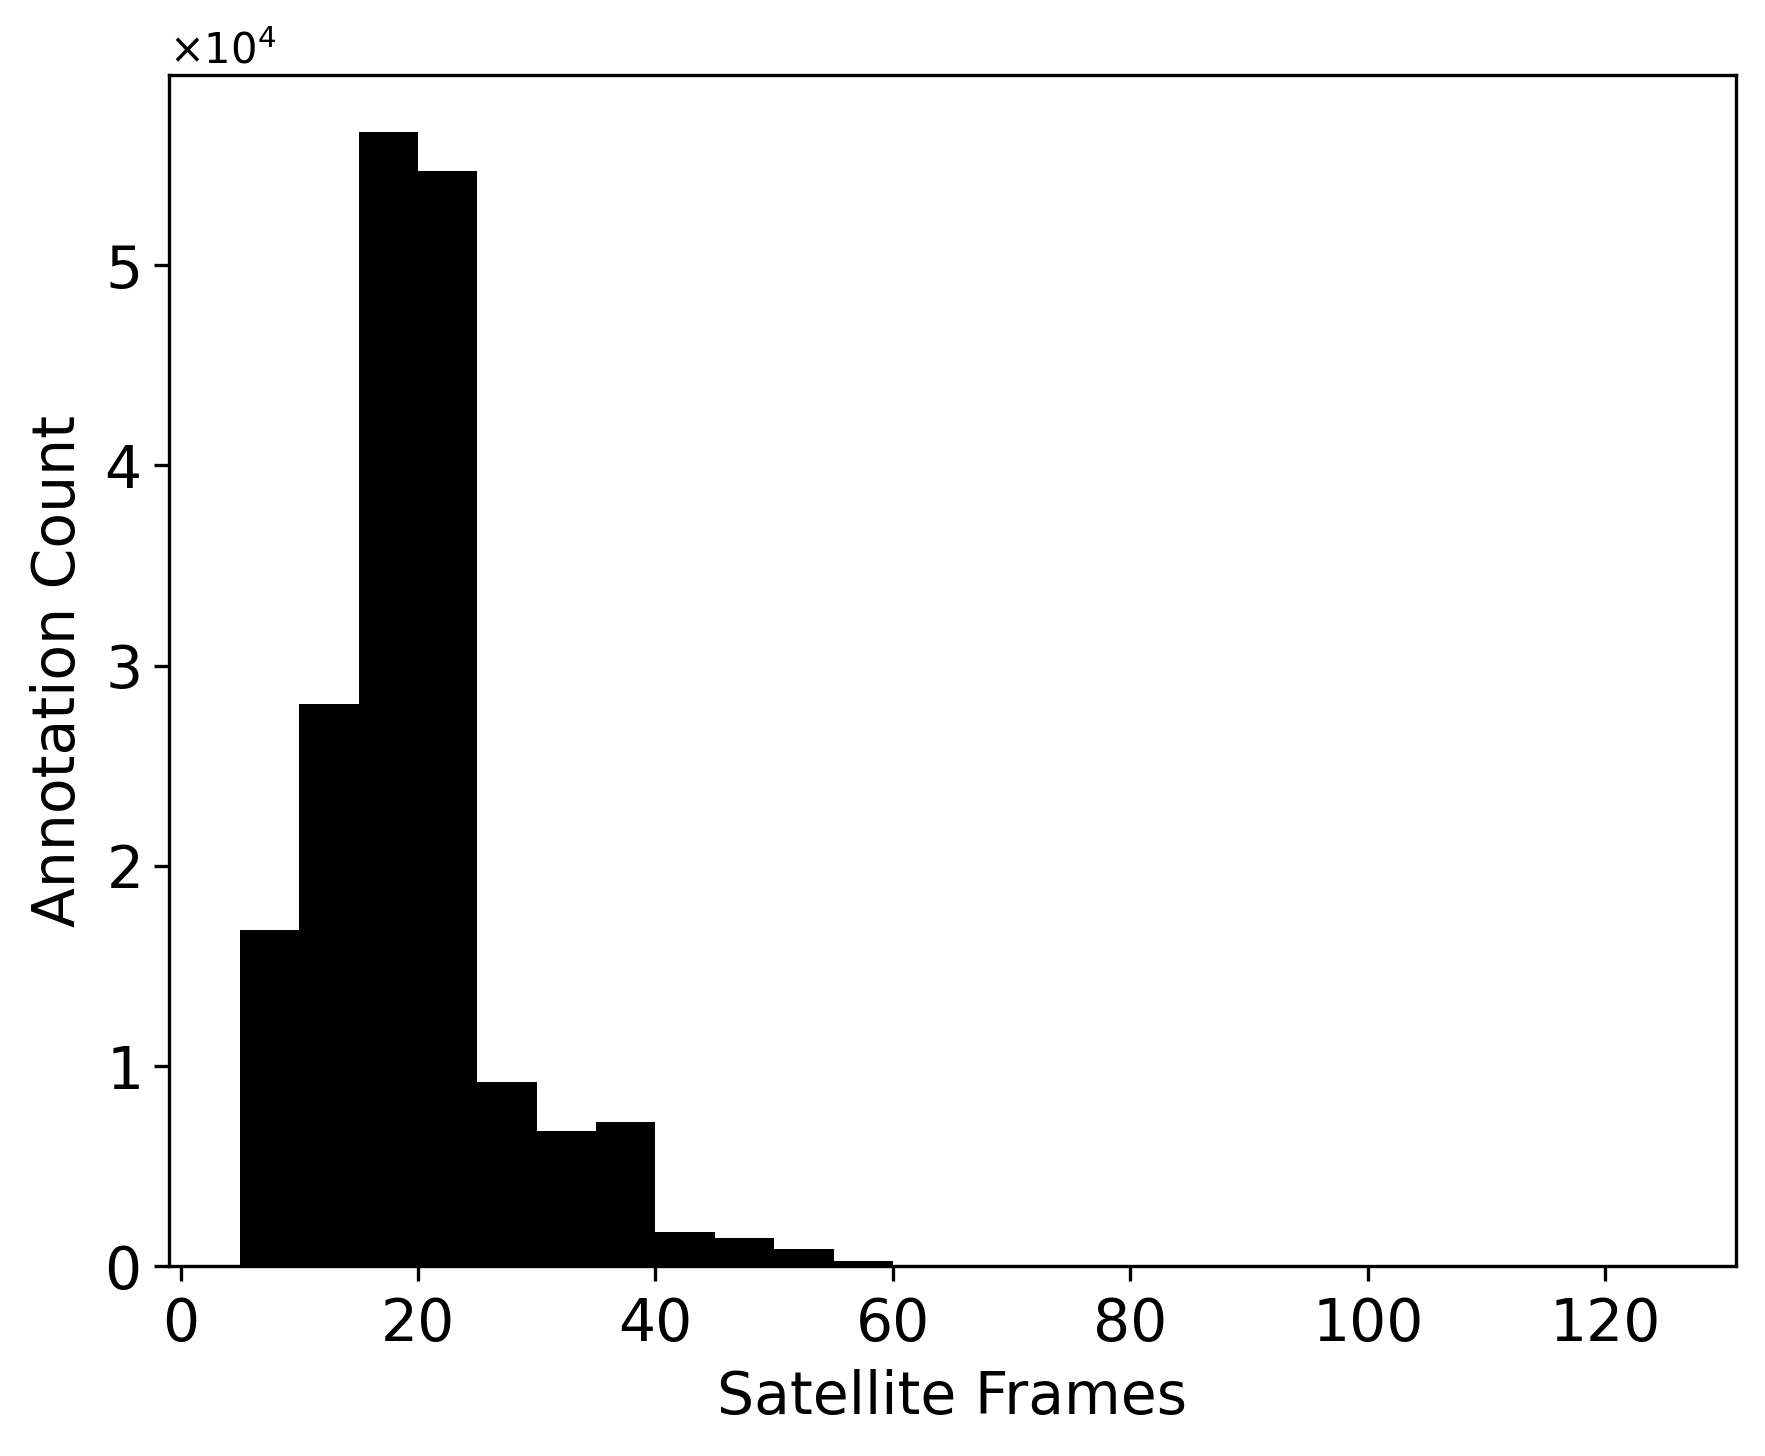
\includegraphics[width=0.49\textwidth]{stat_figs/sample_count_vs_frames.png}
        \caption{The number of annotations that span a number of satellite frames that are generated at a 10-minute interval.}
        \label{num_frames}
\end{figure}

\begin{figure}[!htb]
    \parbox{\textwidth}{
      \parbox{0.49\textwidth}{
        \centering
        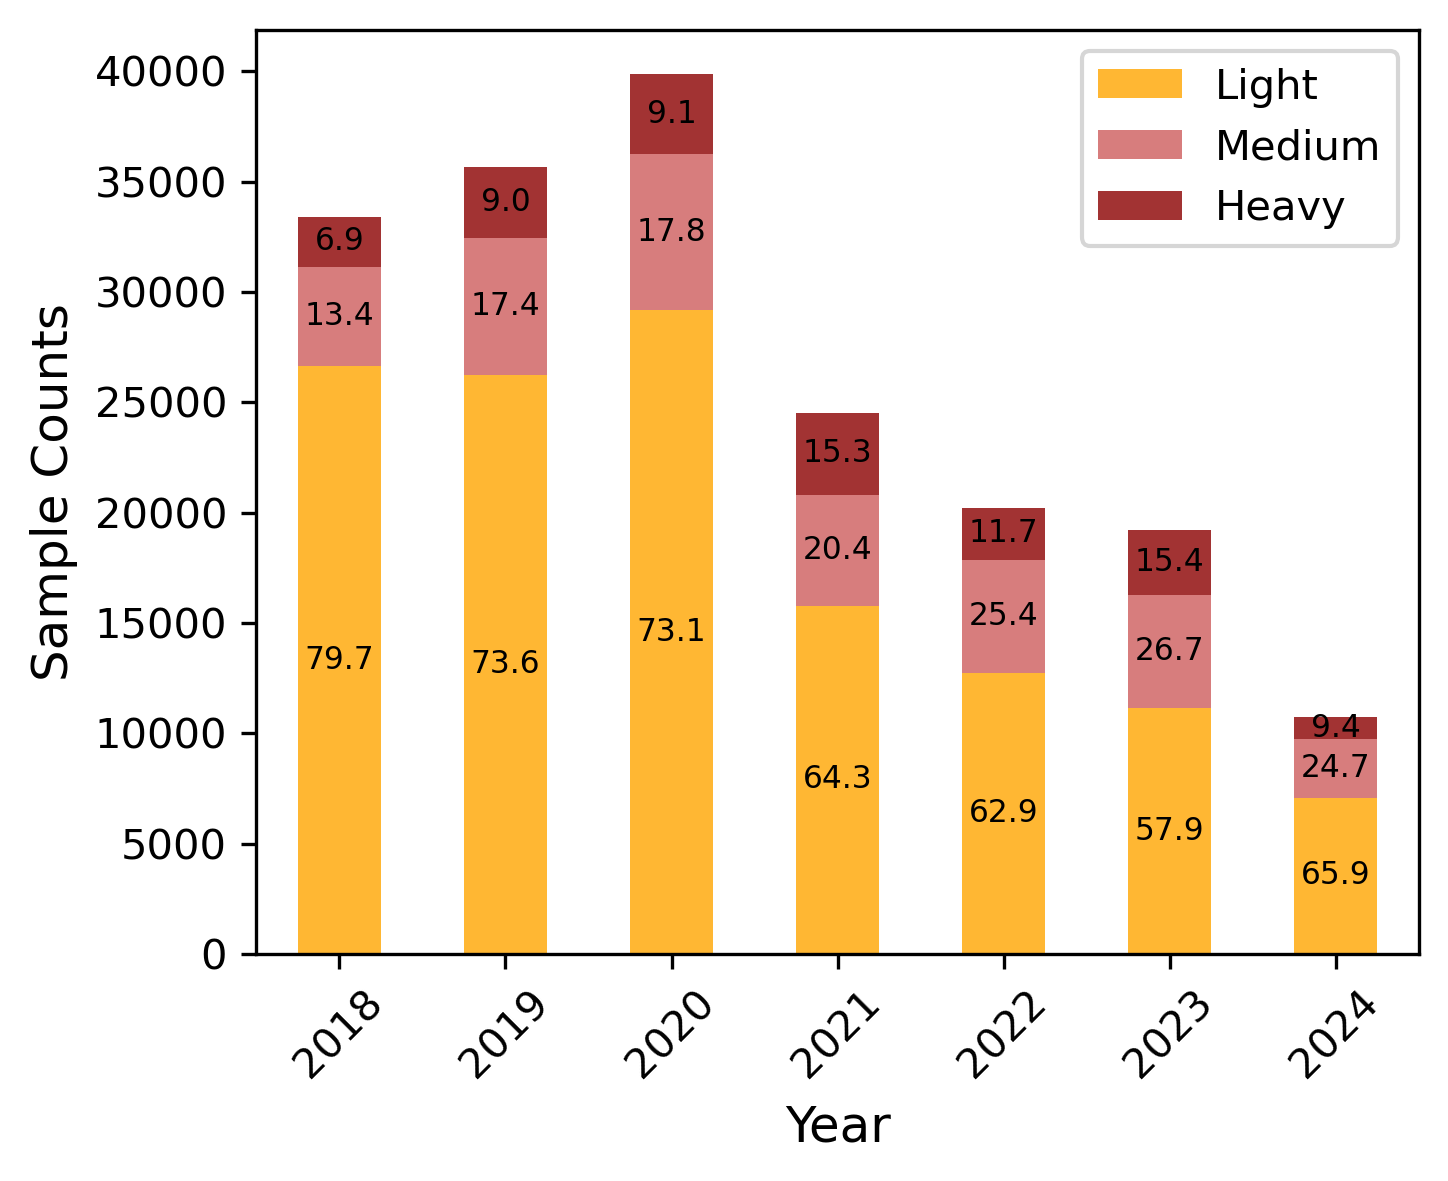
\includegraphics[width=0.49\textwidth]{stat_figs/sample_count_per_yr_percentages.png}
        \caption{Annual sample counts in the SmokeViz dataset, broken down by smoke density class. Percentages within each column indicate the relative frequency of each density level for that year.}
        \label{count_per_yr}
      }
    \hspace{0.01\textwidth}
      \parbox{0.49\textwidth}{
        \centering
        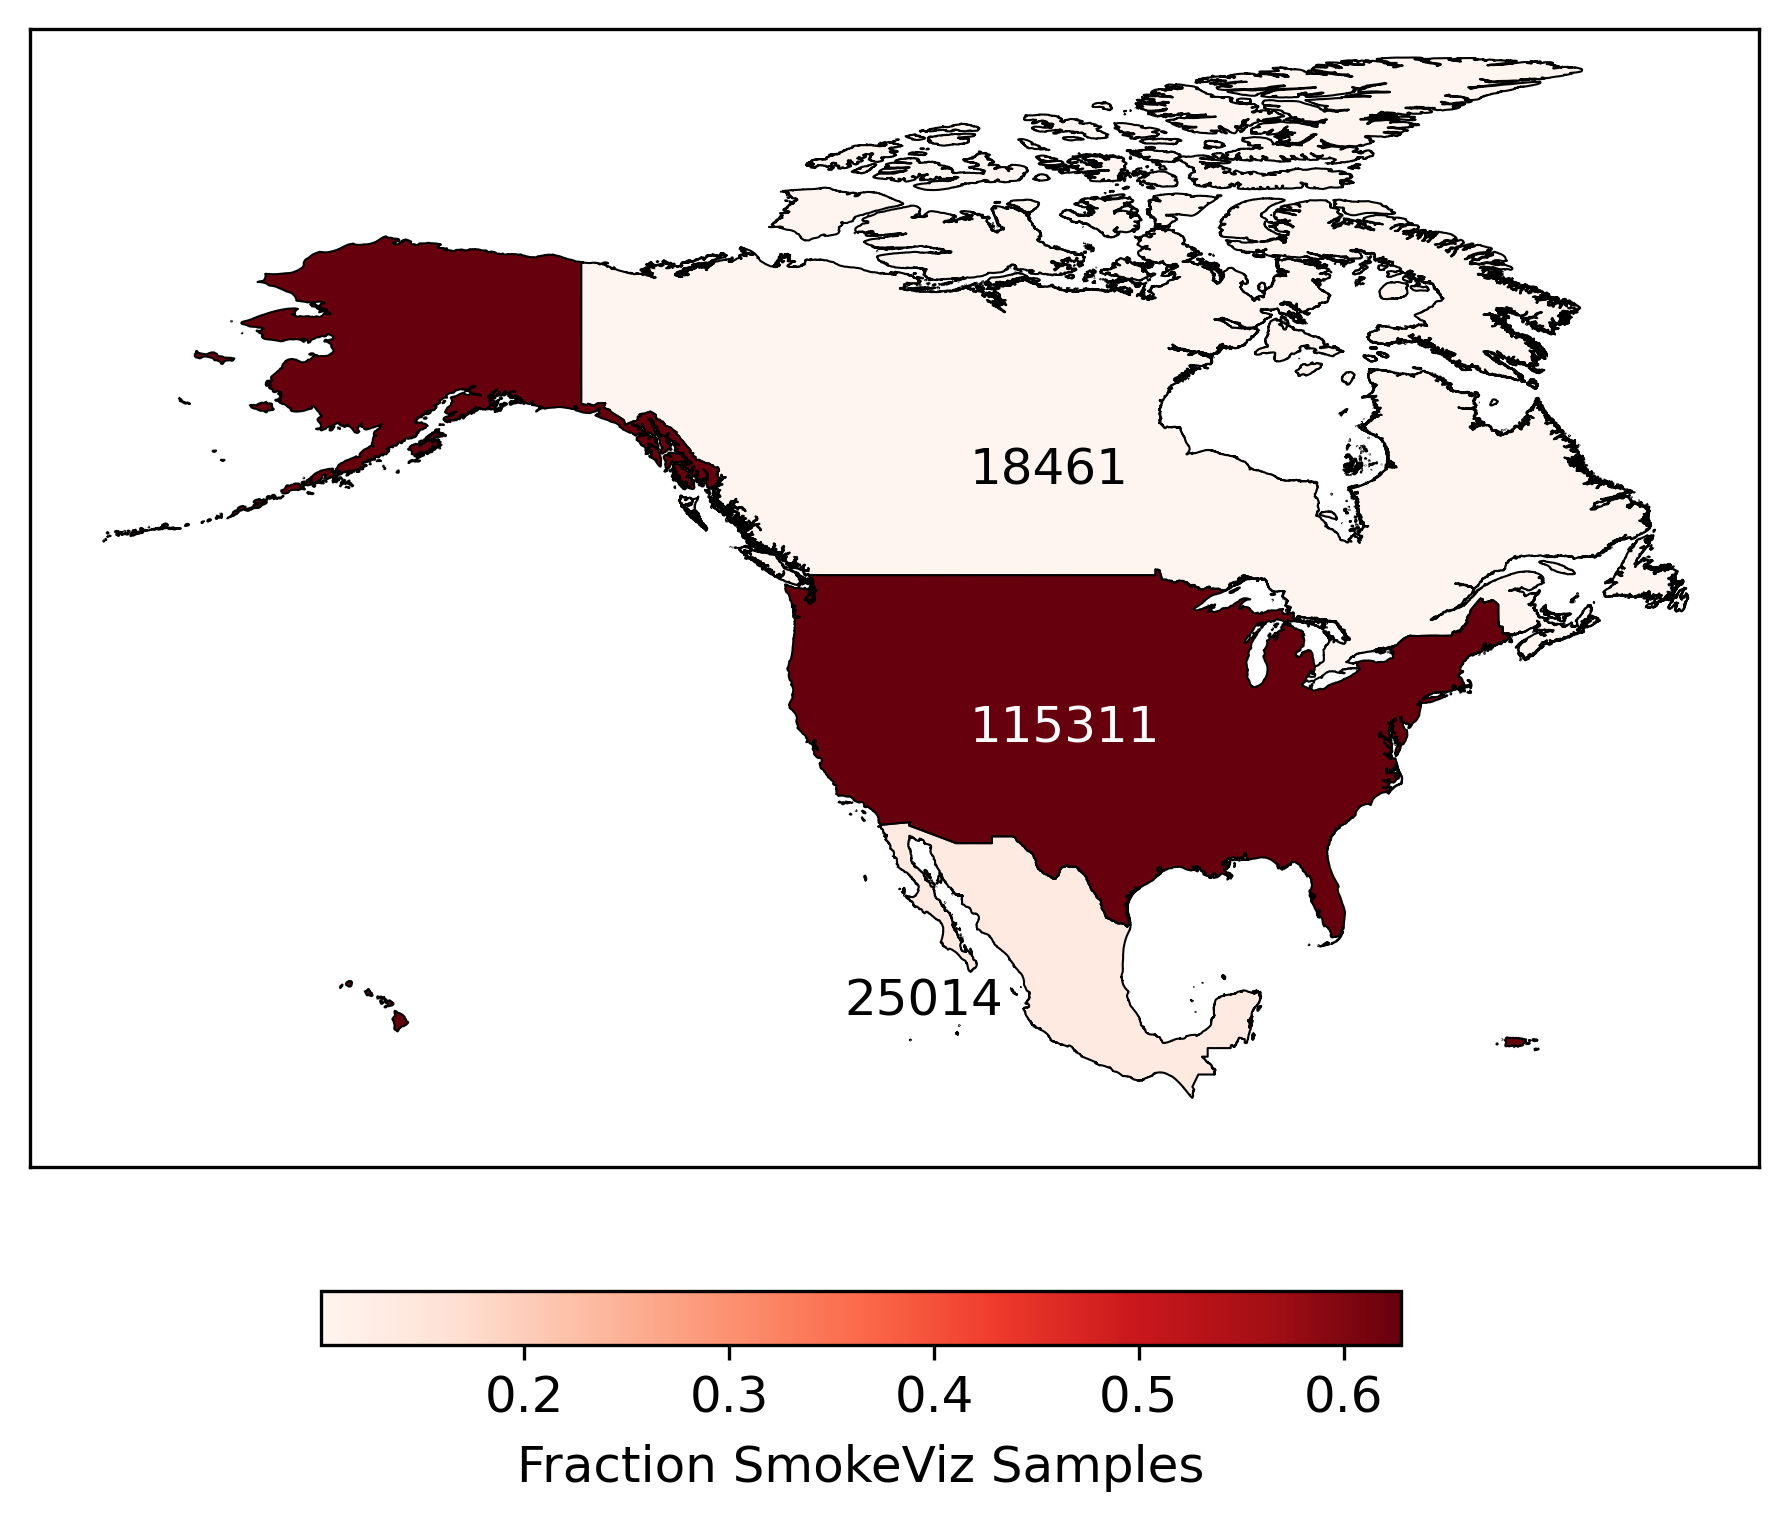
\includegraphics[width=0.49\textwidth]{stat_figs/sample_percent_country.png}
        \caption{Proportion of samples in the SmokeViz dataset whose center pixel falls within Canada, the U.S.A., or Mexico. Sample counts are: Canada: 18,461; U.S.: 115,311; Mexico: 25,014. An additional 24,886 samples are centered over other countries or oceans.}
        \label{count_per_country}
      }
    }
\end{figure}

\subsection{Agricultural Burns}

The monthly peak in sample counts, shown in the main paper (Figure 6), occurs in March and April, preceding the typical wildfire season, which spans from late spring through fall. This early-season spike is likely due to prescribed agricultural burns, which are commonly conducted before vegetation exits winter dormancy \cite{ag_fire}. Since HMS annotations do not distinguish between prescribed burns and wildfires, both event types are included in the dataset.

Model performance over time, also shown in Figure 6, reveals that the highest IoU values for \(f_{c}\) on the \(\mathcal{D}_p\) test set occur during the peak wildfire season (May–September), not during the months with the highest sample counts. This suggests that prescribed burns that are typically smaller and less visually distinct than large wildfires, are more difficult for the model to segment.

A spatial breakdown of sample density further supports this interpretation. Figure 7 in the main paper shows that the states with the highest number of samples are California, Georgia, and Florida. The elevated sample counts in southeastern states are consistent with regional practices of frequent prescribed burns. To investigate regional effects more explicitly, we divide the dataset into four geographic quadrants—Northwest (NW), Southwest (SW), Northeast (NE), and Southeast (SE)—centered around a continental midpoint at \((40^\circ\mathrm{N}, -105^\circ\mathrm{W})\).

Table \ref{quad} reports test IoU and sample counts for each quadrant. Despite containing the largest share of training samples, the Southeast quadrant exhibits the lowest model performance. This degradation is likely due to the abundance of prescribed burns, which may produce smaller, low-opacity smoke plumes that are harder to detect. For users whose objective is to train models specifically for large wildfire detection, this highlights a limitation of the dataset: a substantial portion of the training data originates from controlled burns, which may not be representative of the intended task. One possible mitigation strategy is to filter out short-duration annotations (e.g., single-day events), though this is complicated by variability in analyst-defined time windows and labeling cadence per fire event.


\begin{table}
    \caption{Sample distribution and \(f_{c}\) test performance across geographic quadrants. Despite containing the most data, the Southeast (SE) region yields the lowest IoU.}
    \label{quad}
    \centering
    \begin{tabular}{llll}
        \toprule
        Quadrant & \(\mathcal{D}_p\) Test IoU & \(\mathcal{D}_p\) Test Samples & \(\mathcal{D}_p\) Samples \\
        \midrule
        NW & 0.5887 & 4177 & 32792\\
        SW & 0.4590 & 1937 & 34267\\
        NE & 0.5822 & 1133   & 13342\\
        SE & 0.4798 & 12977 & 103271 \\
        \bottomrule
    \end{tabular}
\end{table}




\subsection{Satellite Analysis}

Figure \ref{sat_dataset} shows the distribution of samples from GOES-East and GOES-West in both the full SmokeViz dataset and the \(\mathcal{D}_p\) test set, along with their respective segmentation performance using \(f_c\). Although GOES-East contributes nearly three-quarters of all samples, model performance is substantially better on GOES-West test samples, with an IoU of 0.6187 compared to 0.4498 for GOES-East.

This discrepancy may stem from several factors. First, the observed signal quality varies between satellites depending on diurnal lighting, seasonal solar angles, and atmospheric conditions. GOES-West best captures forward-scattered sunlight during early morning hours over the western U.S., enhancing smoke visibility via Mie scattering and possibly boosting model accuracy. Additionally, sensor calibration, viewing geometry, and line-of-sight differences between the two platforms could contribute to systematic performance variation.

Another relevant factor is the operational transition between satellites. On June 18, 2022, GOES-17 was replaced by GOES-18 as the operational West satellite. While GOES-17 samples in the test set yield an IoU of 0.6262, GOES-18 samples yield a slightly lower performance at 0.5852. This is likely due to the limited exposure of GOES-18 data during model training: training years (2018–2021) include only GOES-17, while GOES-18 is only present in the 2024 training data. This temporal imbalance may partially explain the drop in IoU for GOES-18.

\begin{figure}[!htb]
    \centering
    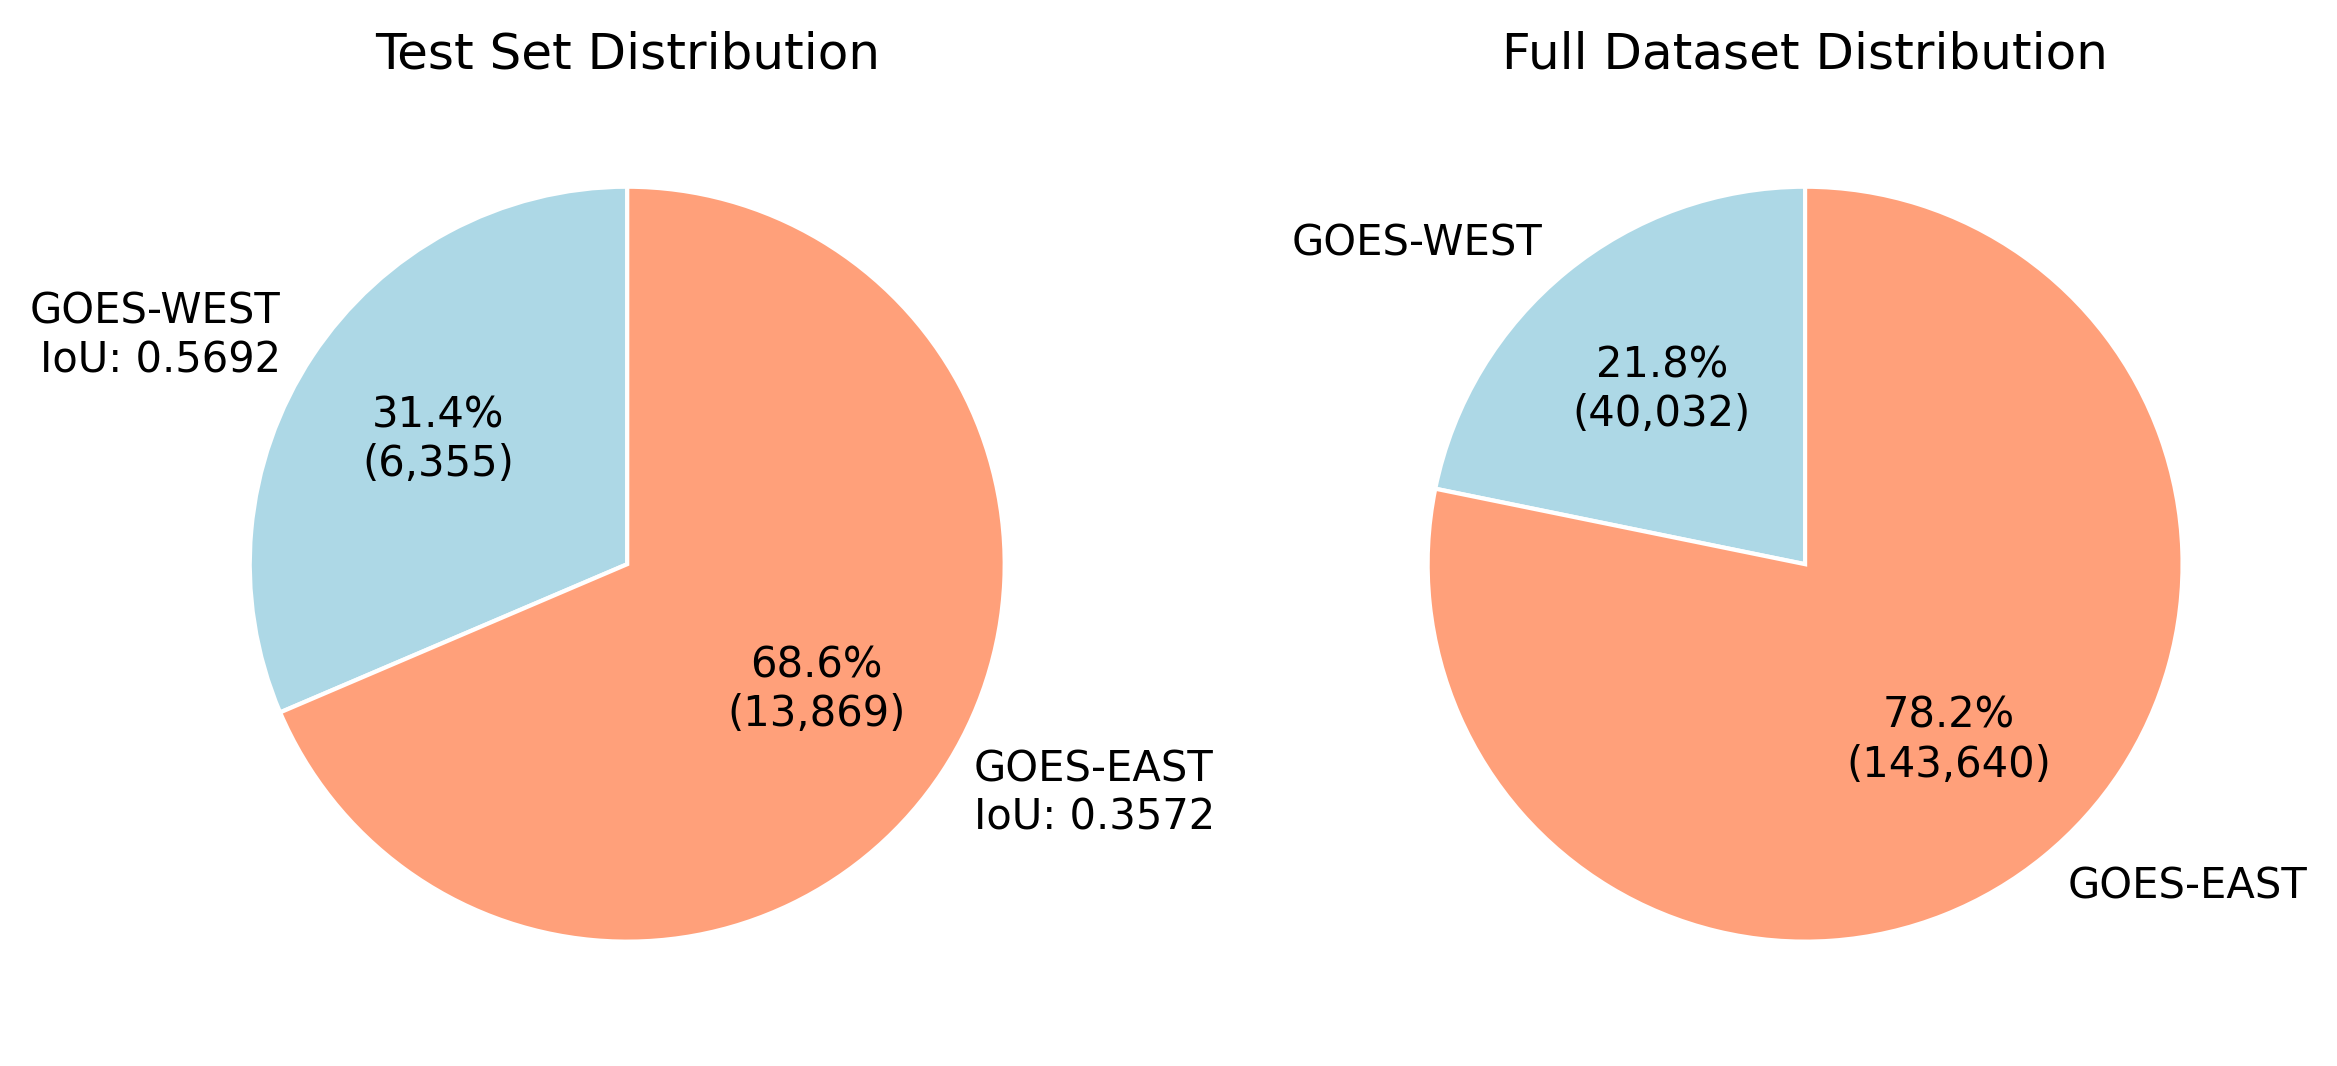
\includegraphics[width=\linewidth]{stat_figs/satellite_test_full_dataset.png}
    \caption{SmokeViz test set (left) and full dataset (right) sample distributions by satellite. GOES-West samples account for a smaller portion of the dataset but yield higher test IoU.}
    \label{sat_dataset}
\end{figure}

\subsection{Sunset/Sunrise Bias}

As mentioned in the limitations, there may have been a bias introduced towards correctly classifying imagery close to sunrise or sunset. This bias may not only be introduced by our Mie-derived dataset that was used to train \(f_{\circ}\), but also in the original HMS annotations. The configuration of the sun, smoke and satellite give the highest signal-to-noise ratio at the times near the sunrise and sunset, making smoke more easily observable by analysts. In contrast, the diurnal variations of wildfires cause the fire radiative power to be highest around solar noon \cite{diurnal}. Table \ref{two_hr_iou} shows how the IoU between \(f_c\) predictions and analyst annotations for the test data from either \(\mathcal{D}_M\) or \(\mathcal{D}_p\) vary based on proximity to sunset/sunrise. One explanation for better values for midday samples could be due to higher amounts of fire activity midday and higher amounts of atmospheric interaction noise early/late in the day. Another difference we see from table \ref{two_hr_iou} is the split of closer to daylight boundaries is shifted towards midday between \(\mathcal{D}_M\) to \(\mathcal{D}_p\). This is because, for \(\mathcal{D}_p\), we are choosing the imagery with the best overlap to the analyst product rather than the image from \(\mathcal{D}_M\) that optimized for highest possible signal-to-noise ratio if given constant signal.

\begin{figure}[!htb]
    \centering
    \includegraphics[width=\linewidth]{stat_figs/Mie_vs_PL_midday.png}
    \caption{Mie Derived dataset vs SmokeViz test sets with IoU}
    \label{DM_vs_DP}
\end{figure}

\begin{figure}[!htb]
    \centering
        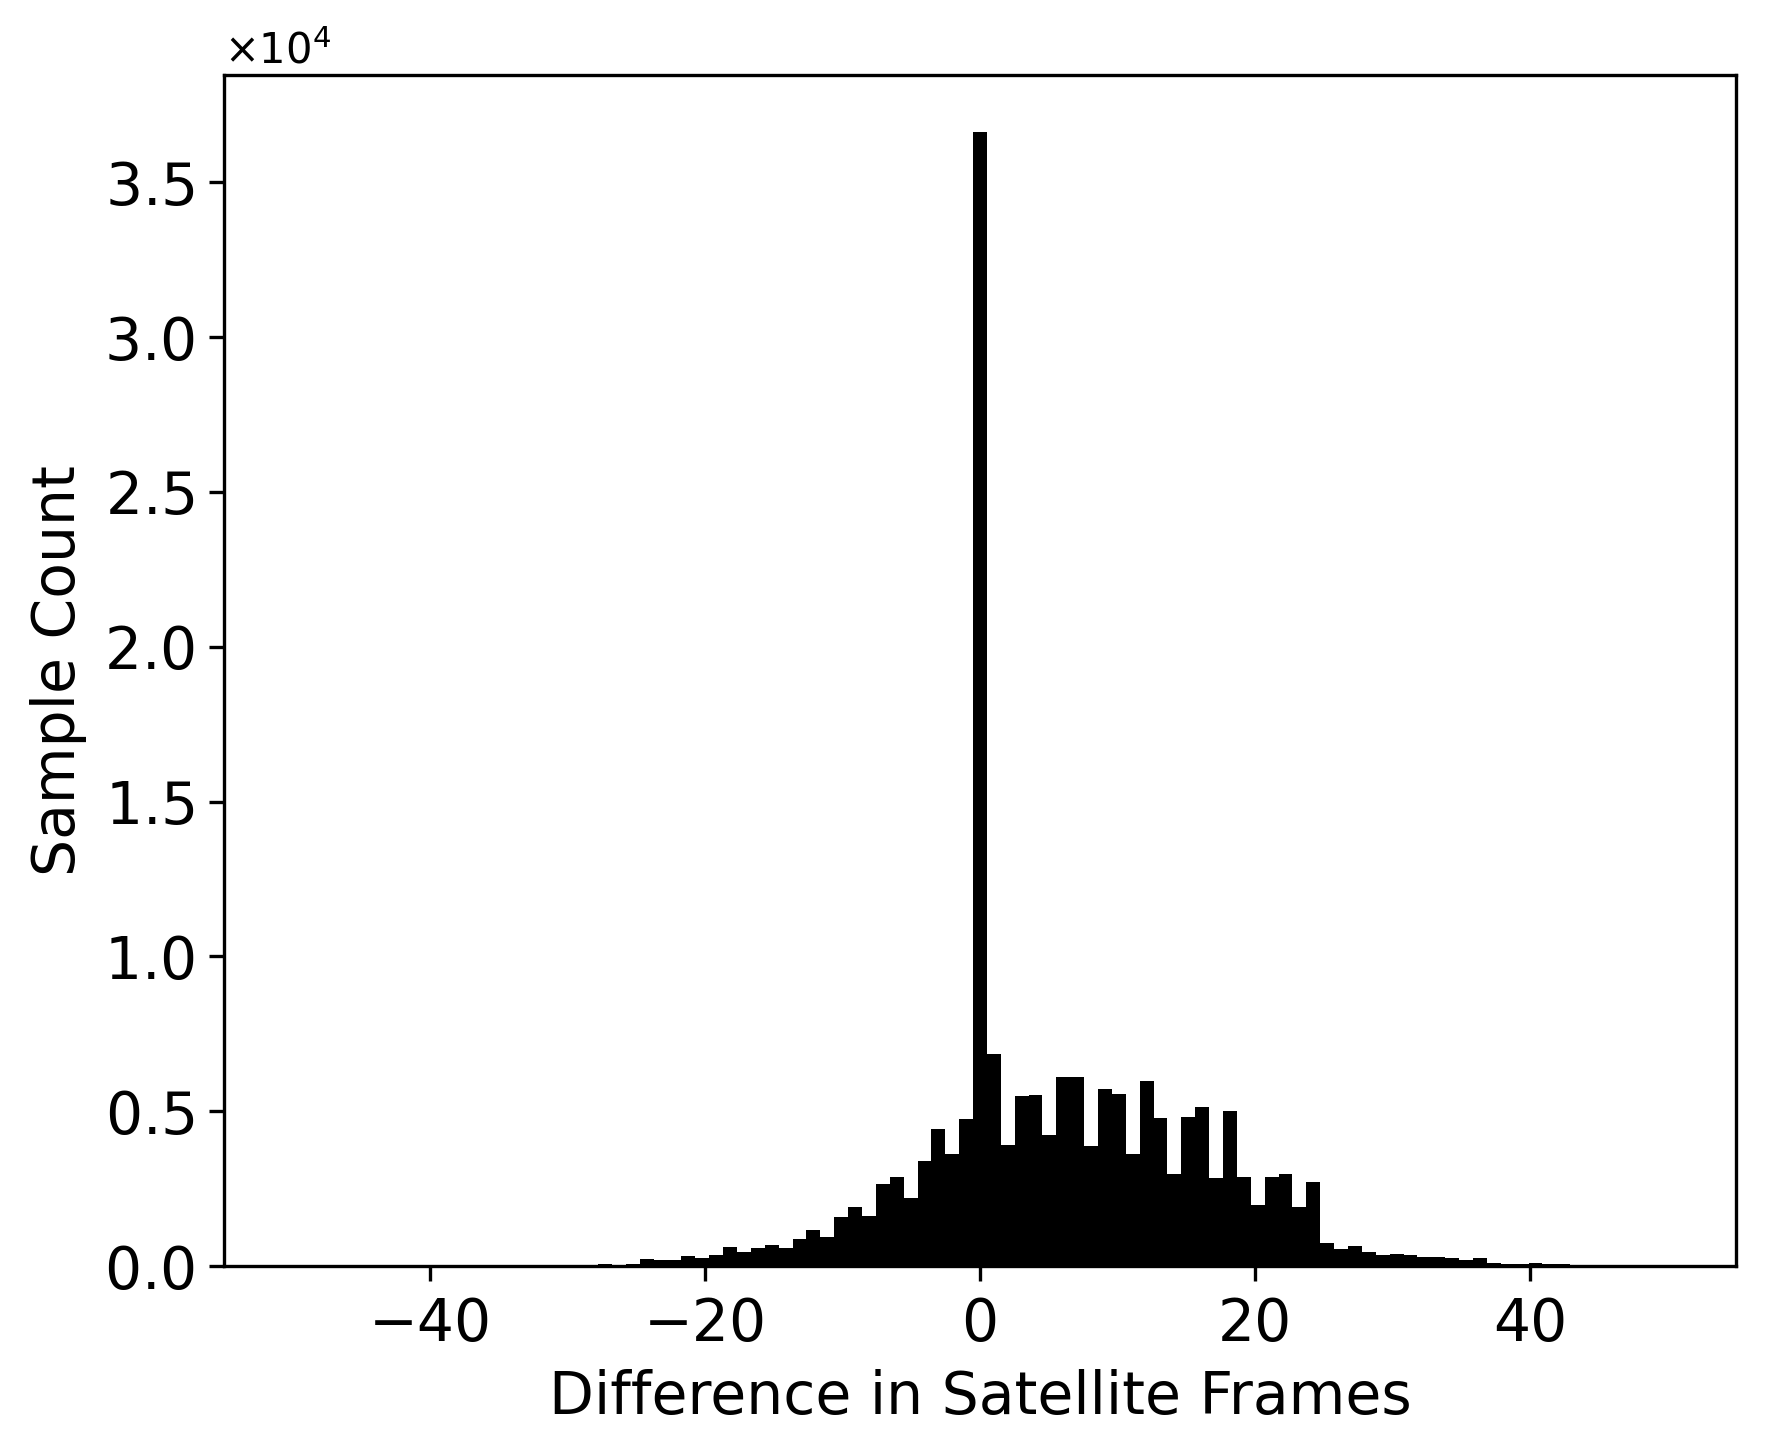
\includegraphics[width=0.49\textwidth]{stat_figs/sample_count_vs_diff_frames.png}
        \caption{The number of satellite frame difference between the \(\mathcal{D}_M\) satellite image and \(\mathcal{D}_p\) chosen satellite image. GOES Full disk images are generated on 10 minute intervals. The number of samples that use the same satellite image in both datasets was 36,608 (\(\approx\)20\%).}
        \label{frame_diff}
\end{figure}



\subsection{Qualitative Analysis on Performance}

Figure \ref{poor} gives some examples of when SmokeViz does not perform well in comparison to the HMS analyst annotations. In the first column example, SmokeViz confuses a smoke-like cloud for smoke, something it generally tends to not seem to have issues with, but this is an counter example to that trend. The second through last columns all miss distinctive plumes that should be classified as either medium or heavy density smoke. In contrast, we show what SmokeViz looks like when it performs well in comparison to the HMS smoke product in figure \ref{good}.

\begin{figure}[!htb]
    \centering
    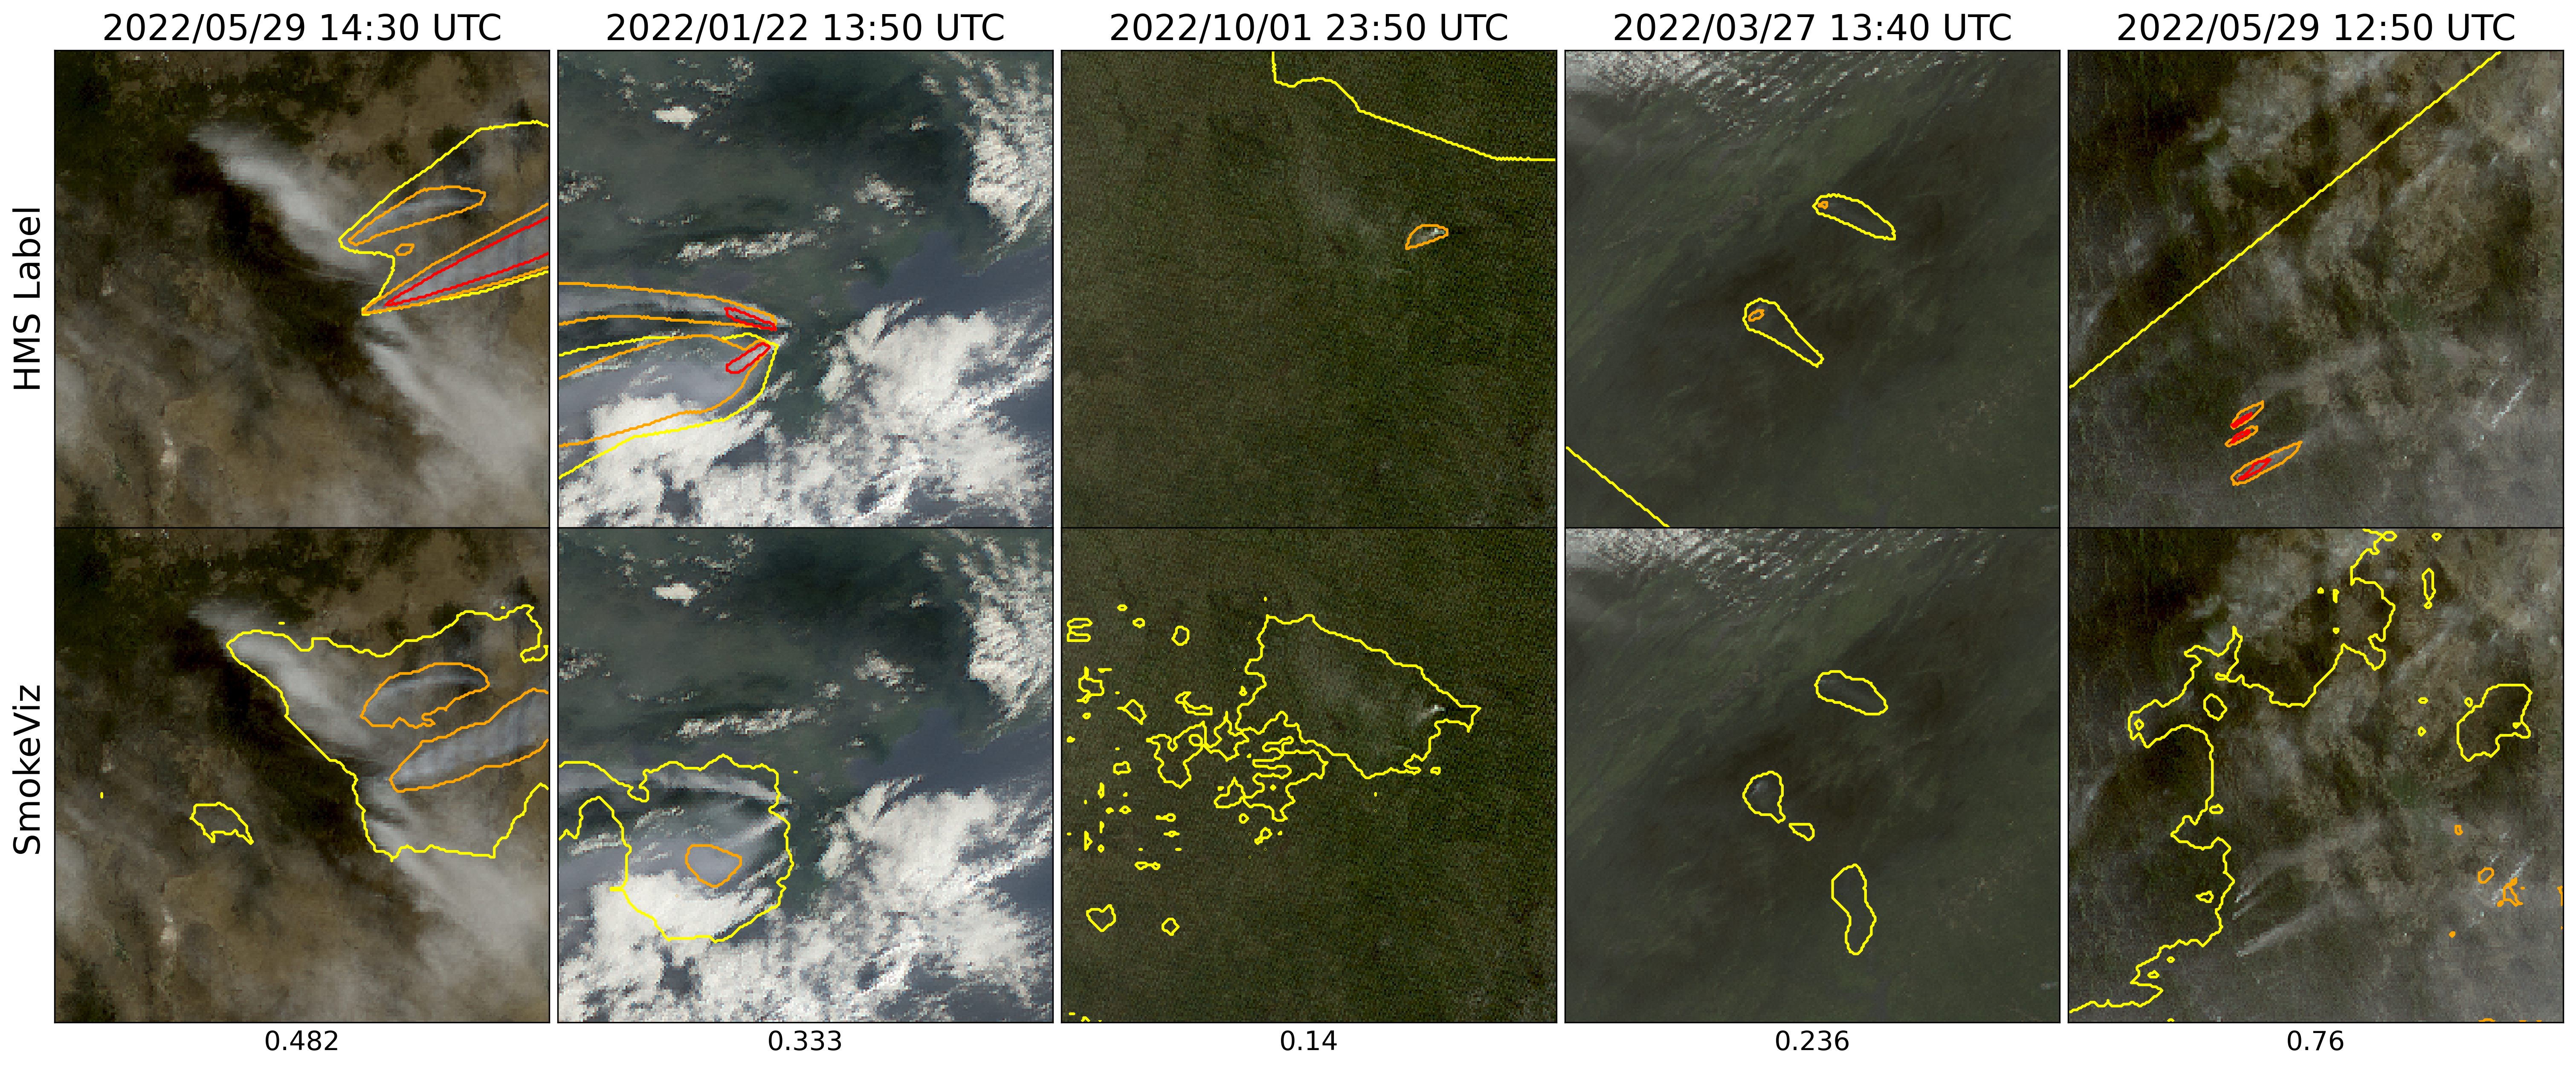
\includegraphics[width=\linewidth]{stat_figs/bad_results.png}
    \caption{Examples of Smoke Viz performing poorly.}
    \label{poor}
\end{figure}


\begin{figure}[!htb]
    \centering
    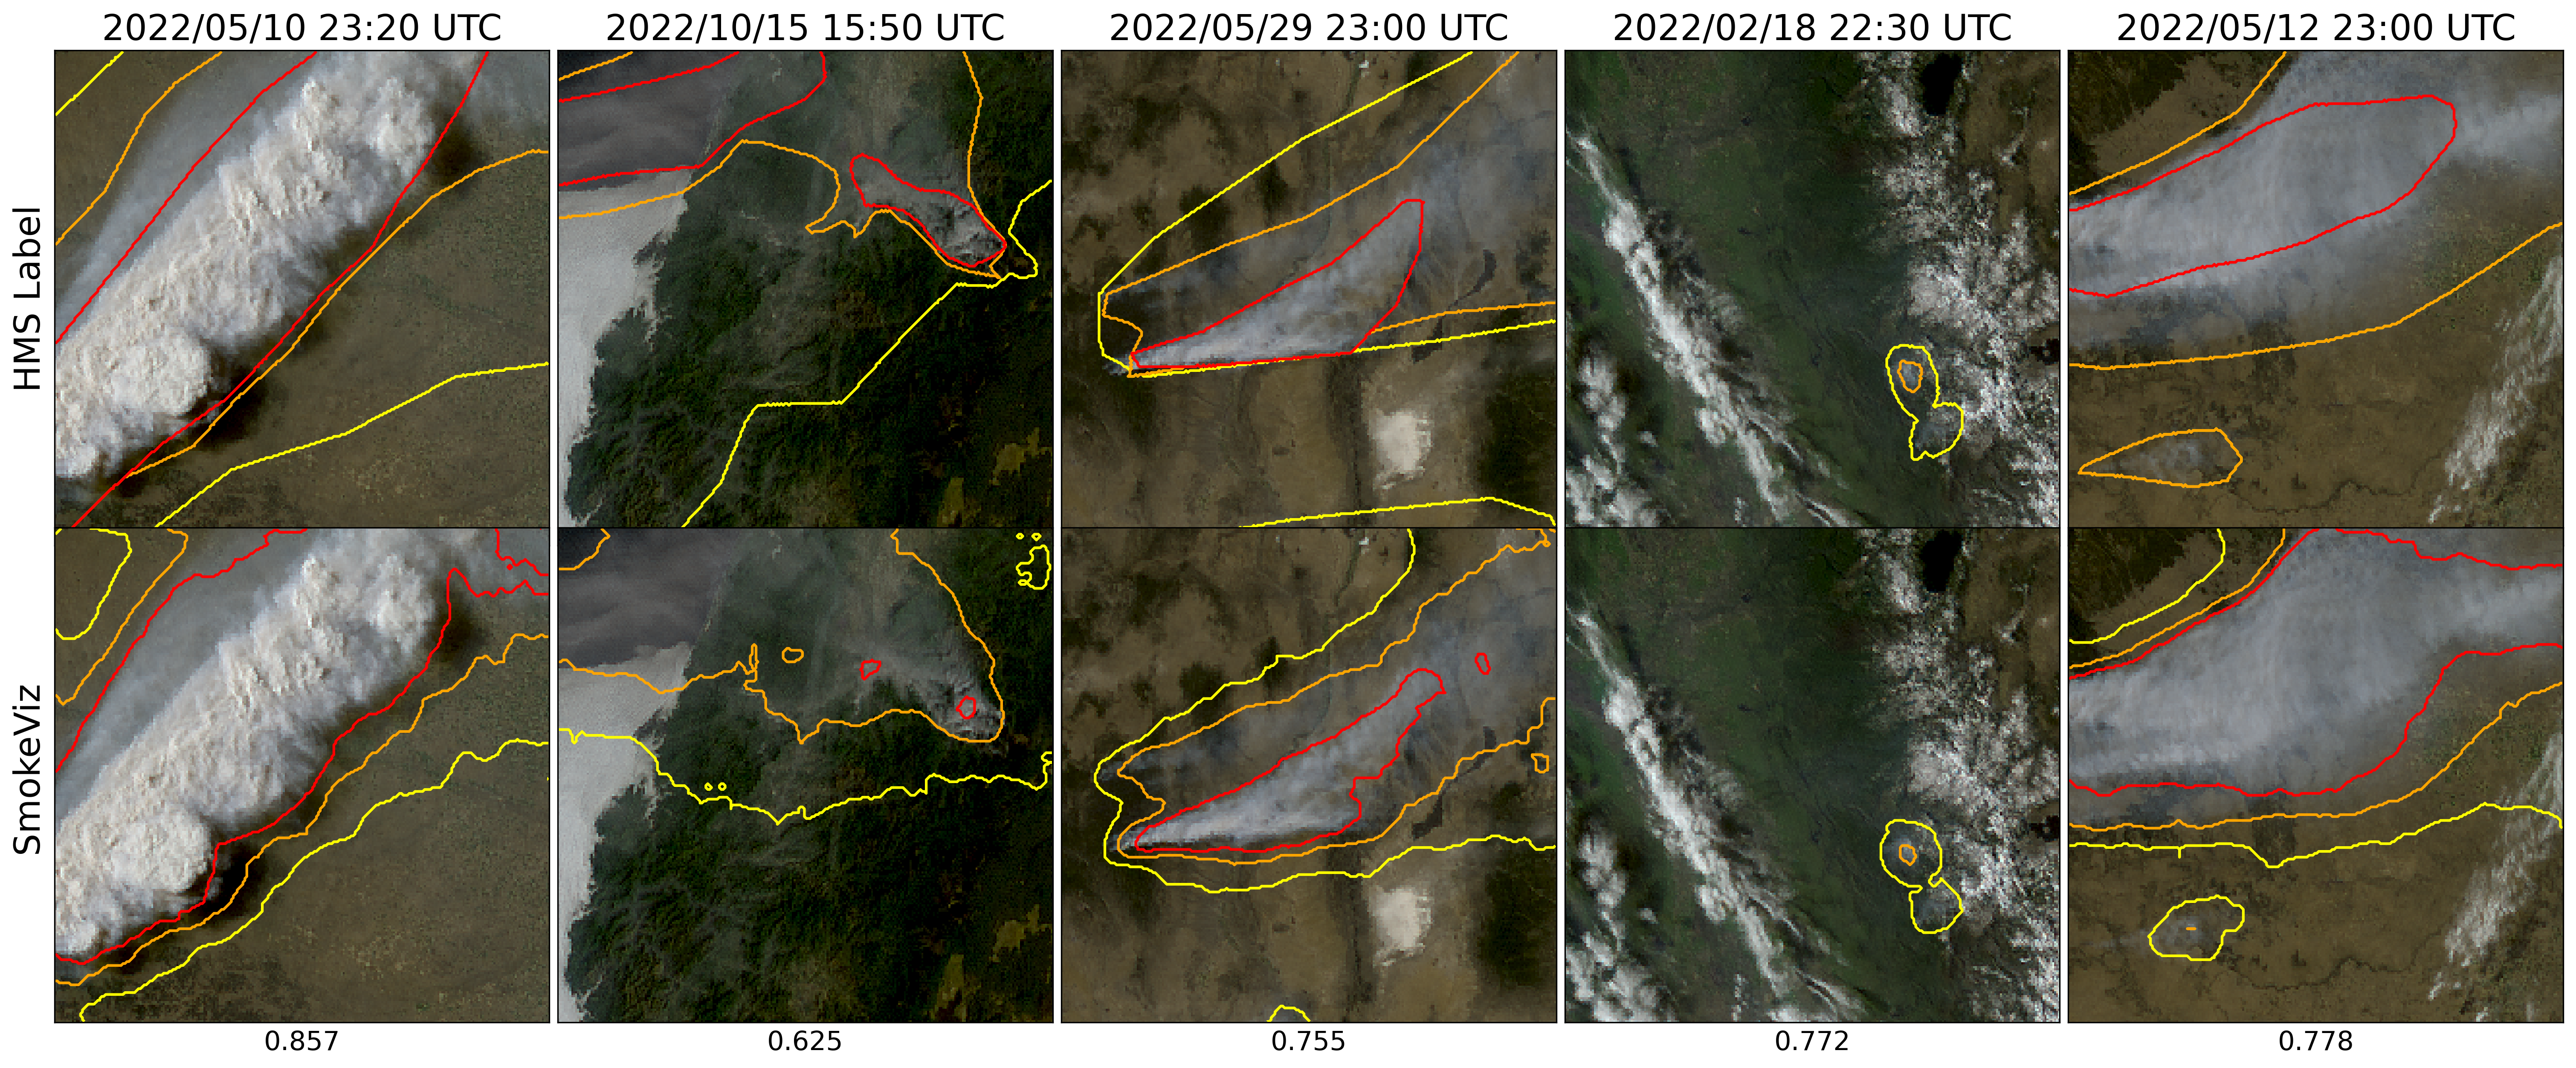
\includegraphics[width=\linewidth]{stat_figs/good_results.png}
    \caption{Examples of Smoke Viz performing well.}
    \label{good}
\end{figure}


\subsection{Machine Learning Reproducibility}

All relevant code is accessible at \url{https://github.com/anonymous-smokeviz/SmokeViz}. The models presented in this paper are not optimized for performance, but are intended to create sufficient pseudo-labels to develop the SmokeViz dataset and then compare the performance of SmokeViz against the original dataset. The child model used in the PLDR process was chosen by running the models shown in table \ref{child} on the Mie-derived dataset and choosing the model with the highest IoU. The hyperparameters used in for the models are shown in table \ref{hyper}. We use the Adam optimizer that will adapt the learning rate during training and is suited for problems with large amounts of data. Batch size was chosen due to the necessity to run the model on limited resources. 

\begin{table}[!htb] 
    \caption{Comparison of segmentation model IoU metrics on the Mie-Derived dataset. Based on the IoU results, the first column that uses EfficientNet and PSPNet was used as for \(f_{\circ}\).}\label{child}
    \centering
    \begin{tabular}{lccccc}
        \toprule
        \textbf{encoder} & EfficientNet\cite{efficientnetv2} & \cite{efficientnetv2} & EfficientViT\cite{efficientvit} & \cite{efficientvit}& ViT \cite{vit} \\
        \textbf{decoder} &  PSPNet\cite{pspnet} & DeepLabV3+\cite{deeplab} & Segformer\cite{segformer} & UperNet \cite{upernet}& DPT\cite{dpt} \\
        \midrule
        Heavy   &	\textbf{0.3221}	& 0.2893	&	0.2185	&	0.3099	&	0.2466 \\
        Medium  &	\textbf{0.4288}	& 0.4091	&	0.3977	&   0.4041	&	0.3135 \\
        Light   &	\textbf{0.5044}	& 0.4424	&	0.4331	&	0.4274	&	0.4964 \\
        Overall &	\textbf{0.4677}	& 0.4172	&   0.4054	&	0.4098	&	0.4331 \\
        \bottomrule
    \end{tabular}
\end{table}

\begin{table}
    \caption{Hyperparameters used to create \(f_{\circ}\) and \(f_{c}\).}
  \label{hyper}
  \centering
  \begin{tabular}{ll}
    \toprule
    parameter & value \\ 
    \midrule
    epochs & 100 \\
    learning rate & 1e-4 \\
    batch size & 16 \\
    optimizer & Adam \\
    \bottomrule
  \end{tabular}
\end{table}


\bibliography{references}
\end{document}
\pagebreak

